\chapter{シミュレーション}
\section{シミュレーション環境}
 このシミュレーションでは,路面を再現するマジックフォーミュラタイヤモデルを使用した. 駆動抵抗は,転がり抵抗,空気抵抗,勾配抵抗で構成される. 各力は式 (27)〜(30)で定式化される.
\begin{flalign}
    F_{\text {roll}}&=-C_{r r} M g \\
    F_{\text {air}}&=-\frac{1}{2} \rho C_{D} S v^{2} \\
    F_{\text {grad}}&=M g \sin \theta_{\text {grad}} \\
    F_{r}&=F_{\text {roll}}+F_{\text {air}}+F_{\text {grad}}
\end{flalign}

\begin{figure}[]
    \centering
    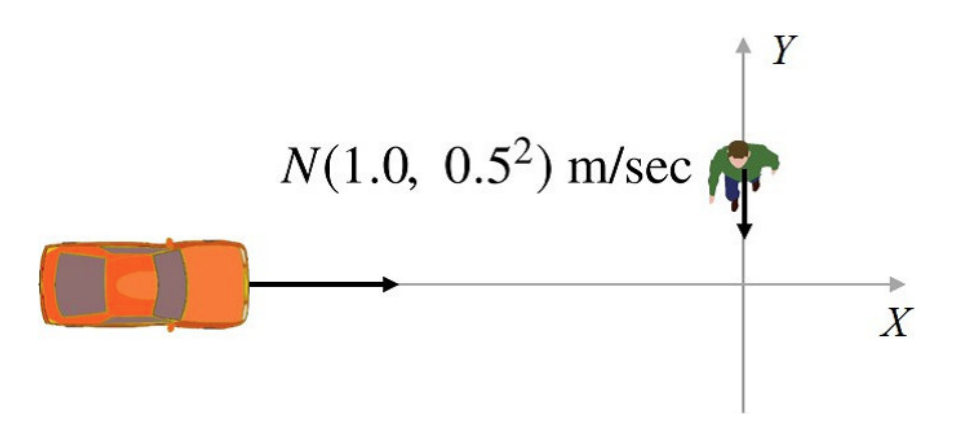
\includegraphics[width=8cm]{./fig/fig7.png}
    \caption{シミュレーションの状況}
\end{figure}

\begin{table}[]
    \centering
    \caption{シミュレーションでの道路環境}
    \begin{tabular}{|c|c|c|}
    \hline
    Road & Surface & Gradient \\ \hline
    1    & Dry     & Downhill \\ \hline
    2    & Wet     & Flat     \\ \hline
    \end{tabular}
\end{table}

\begin{table}[htbp]
    \centering
    \caption{シミュレーション条件}
    \scalebox{0.87} {
        \begin{tabular}{|c|c|c|}
            \hline
            Parameter                                  & Value   & Unit     \\ \hline
            Vehicle mass $M$                           & 1000    & kg       \\ \hline
            Wheel radius $r_{\omega}$                  & 0.302   & m        \\ \hline
            Number of controlled wheels $n$            & 4       &          \\ \hline
            Motor Inertia $J_{\omega h}$               & 1.24    & kgm$^2$  \\ \hline
            Motor viscosity coefficient $D_{\omega h}$ & 0.00040 & Nsec/m   \\ \hline
            Motor coulomb friction $f_{\omega h}$      & 0.001   &          \\ \hline
            Sample time in MPC $T_s$                   & 0.1     & sec      \\ \hline
            Integral gain $K_i$                        & 50000   &          \\ \hline
            prediction horizon $H_p$                   & 30      &          \\ \hline
            Control horizon $H_u$                      & 10      &          \\ \hline
            Safety zone for pedestrian $R_h$           & 0.5     &          \\ \hline
            Downhill gradient $\theta_p$               & 5       & deg      \\ \hline
            Rolling resistance coefficient $C_{rr}$    & 0.01    &          \\ \hline
            Air resistance coefficient $C_d$           & 0.3     &          \\ \hline
            Projected area $S$                         & 1.754   & m$^2$    \\ \hline
            Air density $\rho$                         & 1.225   & kg/m$^3$ \\ \hline
        \end{tabular}
    }
\end{table}

 シミュレーションパラメータを表3に示す.シミュレーション1では,道路環境1での走行時に走行抵抗が補正されるかどうかの比較を行う.さらに,道路環境2では路面での最大摩擦係数の推定の有無について比較を行う.

\section{シミュレーション結果}
 シミュレーション1の結果を図8と〜図10に示す.図8は,車両と歩行者の位置を示している. 図8によると,システムは良好に機能し,車両は運転抵抗を補償することで歩行者の前方に停止した. 走行抵抗補正がない場合,車両は歩行者の前で停止できなかった. したがって,駆動抵抗を補償することが検証された.\\
 また,図9は,推定値と駆動抵抗の真値との比較を示しており,値が真値に近づいたことを示している.図10から提案手法で適切な制動力が発生していることを確認できる.補償付き制御法を利用する場合は,駆動力を考慮した制動力を車両に追加する.道路環境1は下り坂であり,走行抵抗には正の勾配抵抗が含まれる.したがって,司令位置で停止するには,車両を強くブレーキする必要がある.\\
 同様に,シミュレーション2の結果を図11〜図13に示す.\\
 図11は,車両と歩行者の位置を示している.図11によれば,路面が濡れていても最大摩擦係数を推定することにより,車両は歩行者の前方を停止した.図12は最大摩擦係数の推定結果を示しており,推定値が真の値よりわずかに小さい値に収束したことを示している.図10から提案手法で適切な制動力が発生することが確認された.最大摩擦係数を推定しない場合,タイヤ力の絶対値は2.4秒から減少した.これは,制動力が摩擦円理論の制限を超え,タイヤがスリップしたことを示している.したがって,推定最大摩擦係数に対する有効性が確認された.
\newpage

\begin{figure}[H]
    \centering
    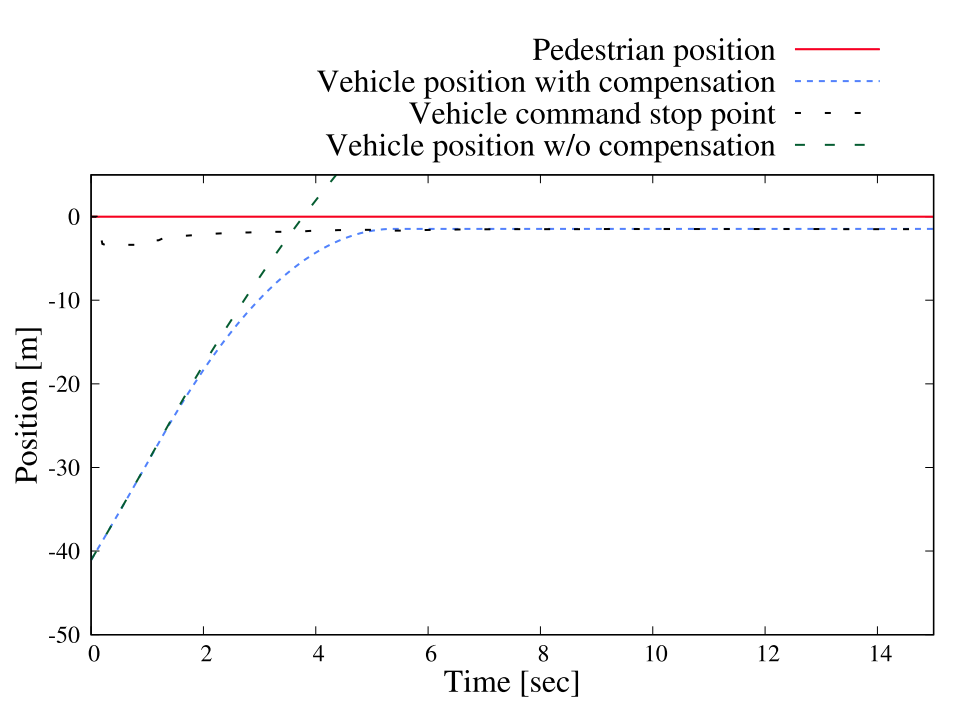
\includegraphics[width=8cm]{./fig/fig8.png}
    \caption{車両位置のシミュレーション1結果}
\end{figure}

\begin{figure}[H]
    \centering
    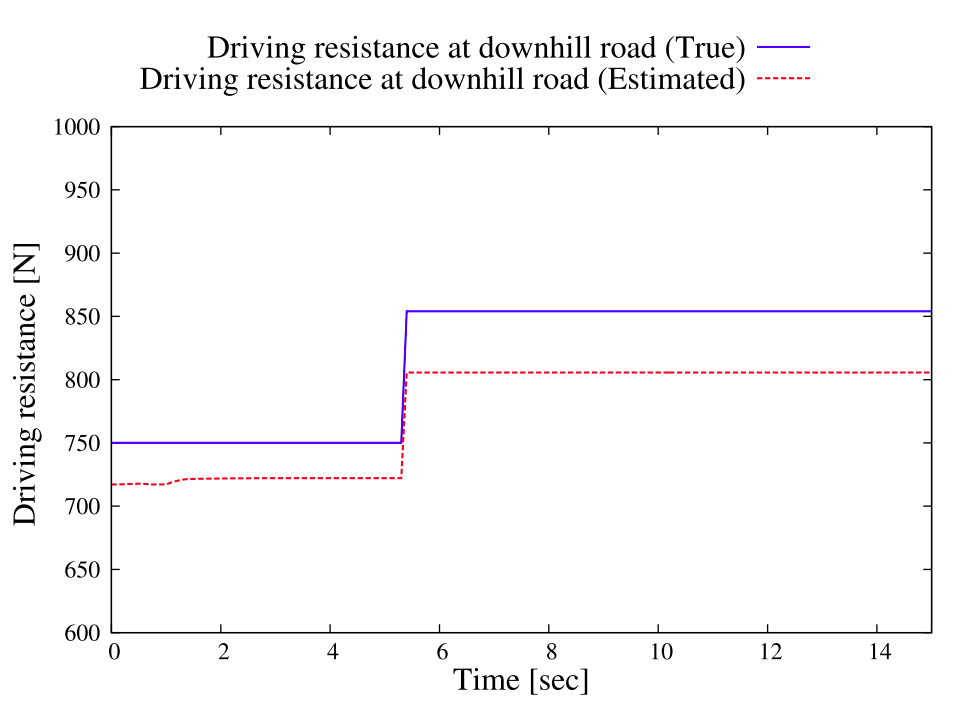
\includegraphics[width=8cm]{./fig/fig9.png}
    \caption{運転抵抗のシミュレーション1結果}
\end{figure}

\begin{figure}[H]
    \centering
    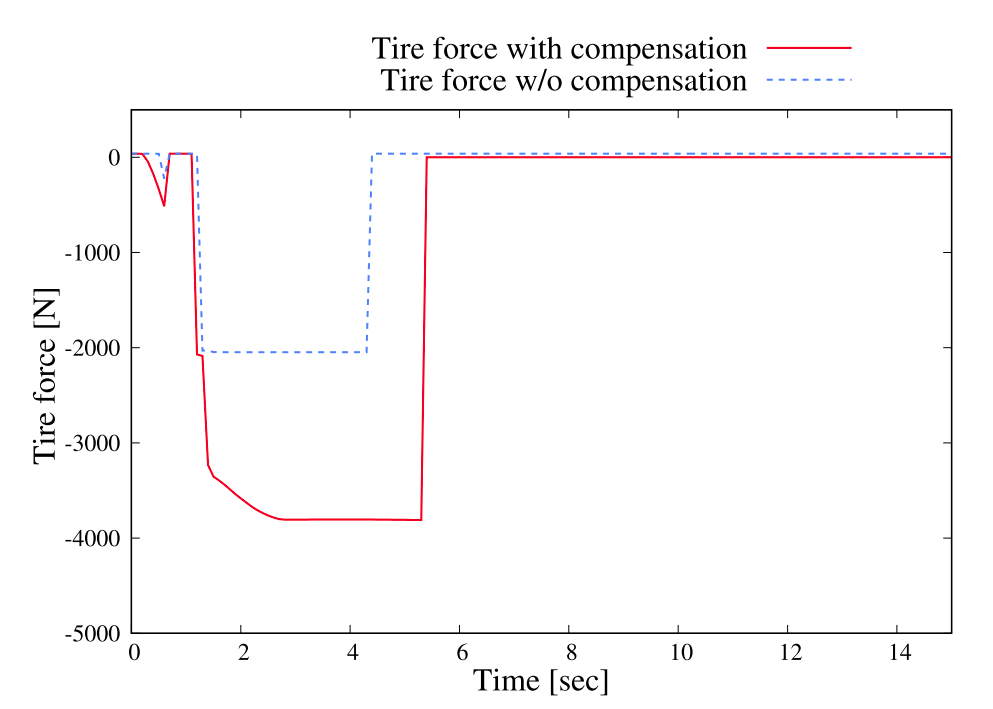
\includegraphics[width=8cm]{./fig/fig10.png}
    \caption{タイヤ力のシミュレーション1結果}
\end{figure}
\newpage
\begin{figure}[H]
    \centering
    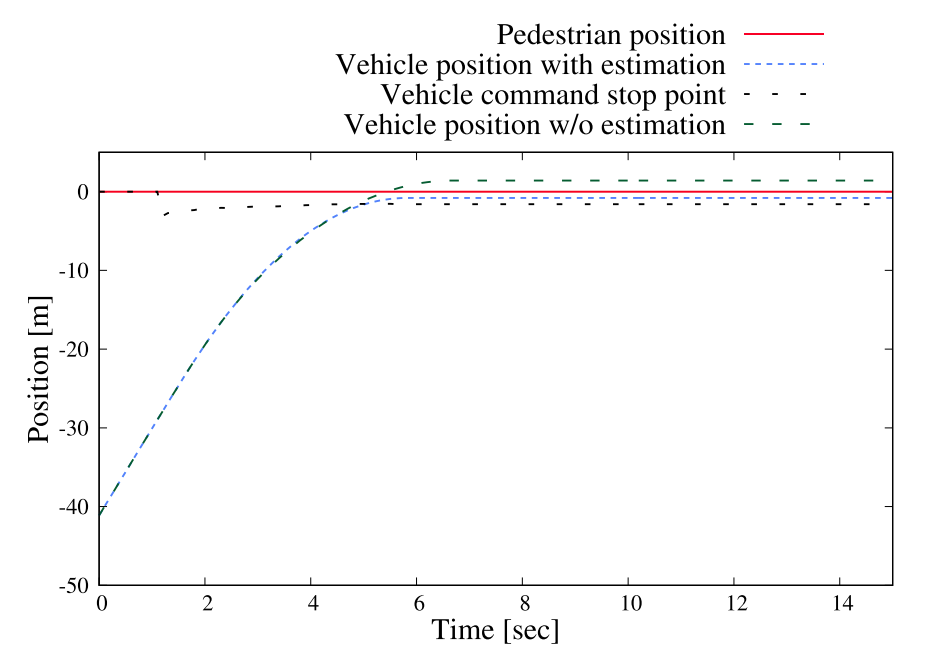
\includegraphics[width=8cm]{./fig/fig11.png}
    \caption{車両位置のシミュレーション2結果}
\end{figure}

\begin{figure}[H]
    \centering
    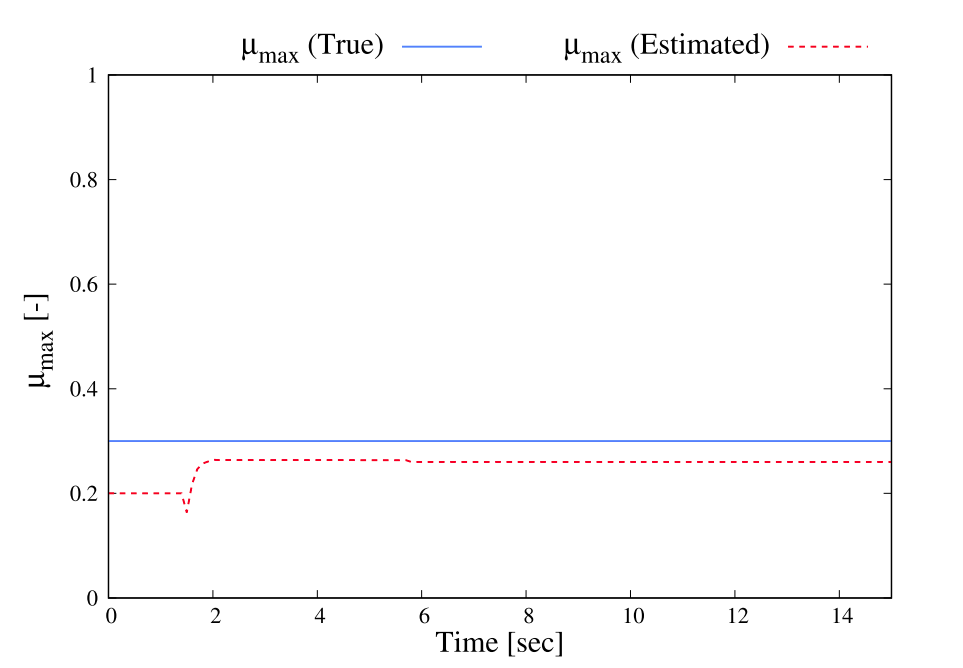
\includegraphics[width=8cm]{./fig/fig12.png}
    \caption{運転抵抗のシミュレーション2結果}
\end{figure}

\begin{figure}[H]
    \centering
    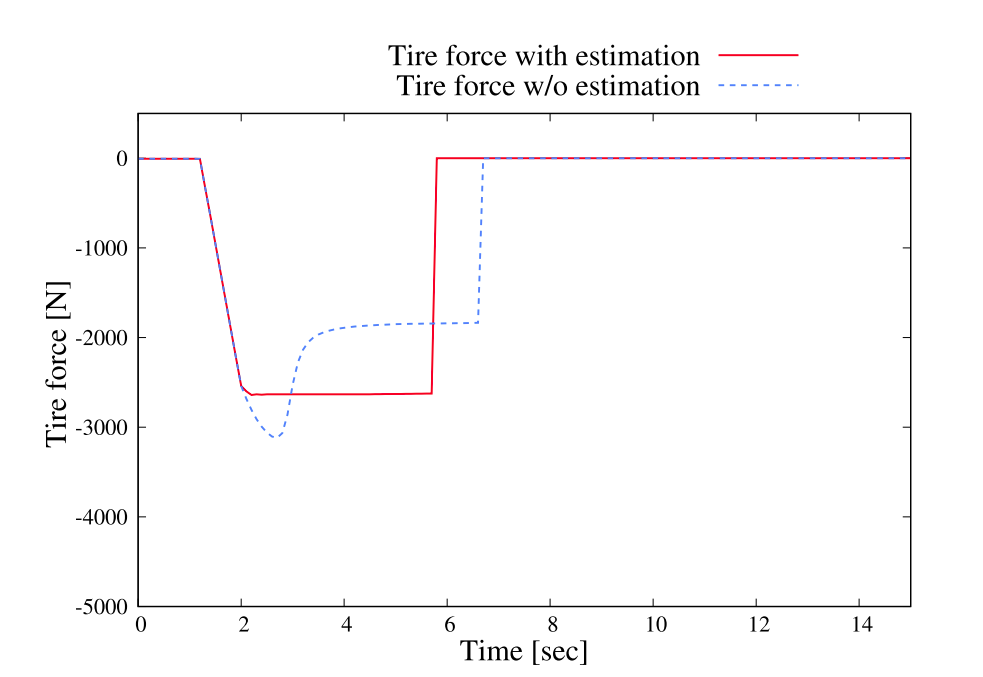
\includegraphics[width=8cm]{./fig/fig13.png}
    \caption{タイヤ力のシミュレーション2結果}
\end{figure}
